\documentclass{article}
\usepackage[utf8]{inputenc} % Required for inputting international characters
\usepackage[T1]{fontenc} % Output font encoding for international characters

%%%%%%%%%%%%%%%%%%%%%%%%%%%%%%%%%
% PACKAGE IMPORTS
%%%%%%%%%%%%%%%%%%%%%%%%%%%%%%%%%
\usepackage[tmargin=2cm,rmargin=1in,lmargin=1in,margin=0.85in,bmargin=2cm,footskip=.2in]{geometry}
\usepackage{amsmath,amsfonts,amsthm,amssymb,mathtools} %general maths stuff
\usepackage[varbb]{newpxmath} %maths tools
\usepackage{xfrac} %a/b fractions
\usepackage[makeroom]{cancel}
\usepackage{mathtools}
\usepackage{bookmark}
\usepackage{enumitem}
\usepackage{hyperref,theoremref}
\hypersetup{
	pdftitle={Past Paper},
	colorlinks=true, linkcolor=black!90,
	bookmarksnumbered=true,
	bookmarksopen=true
}
\usepackage[most,many,breakable]{tcolorbox}
\usepackage{xcolor}
\usepackage{varwidth}
\usepackage{varwidth}
\usepackage{etoolbox}
\usepackage{nameref}
\usepackage{multicol,array}
\usepackage{tikz-cd}
\usepackage[ruled,vlined,linesnumbered]{algorithm2e}
\usepackage{comment} % enables the use of multi-line comments (\ifx \fi) 
\usepackage{import}
\usepackage{xifthen}
\usepackage{pdfpages}
\usepackage{transparent}
\usepackage{tikzsymbols}

\usepackage[default]{raleway}
\usepackage{sectsty}
\renewcommand*\familydefault{\sfdefault} % Force the sans-serif version of any font used
\allsectionsfont{\sffamily\mdseries\upshape} % (See the fntguide.pdf for font help)

\usepackage[nottoc,notlof,notlot]{tocbibind} % Put the bibliography in the ToC
\usepackage[titles,subfigure]{tocloft} % Alter the style of the Table of Contents
\renewcommand{\cftsecfont}{\rmfamily\mdseries\upshape}
\renewcommand{\cftsecpagefont}{\rmfamily\mdseries\upshape} % No bold!

\usepackage{calc}
\usepackage{subfig}
\usepackage{pgfplots}
\pgfplotsset{compat = newest}


%%%%%%%%%%%%%%%%%%%%%%%%%%%%%%J
% SELF MADE COLORS
%%%%%%%%%%%%%%%%%%%%%%%%%%%%%%

\definecolor{myg}{RGB}{56, 140, 70}
\definecolor{myb}{RGB}{45, 111, 177}
\definecolor{myr}{RGB}{199, 68, 64}
\definecolor{mytheorembg}{HTML}{F2F2F9}
\definecolor{mytheoremfr}{HTML}{00007B}
\definecolor{mylenmabg}{HTML}{FFFAF8}
\definecolor{mylenmafr}{HTML}{983b0f}
\definecolor{mypropbg}{HTML}{f2fbfc}
\definecolor{mypropfr}{HTML}{191971}
\definecolor{myexamplebg}{HTML}{F2FBF8}
\definecolor{myexamplefr}{HTML}{88D6D1}
\definecolor{myexampleti}{HTML}{2A7F7F}
\definecolor{mydefinitbg}{HTML}{E5E5FF}
\definecolor{mydefinitfr}{HTML}{3F3FA3}
\definecolor{notesgreen}{RGB}{0,162,0}
\definecolor{myp}{RGB}{197, 92, 212}
\definecolor{mygr}{HTML}{2C3338}
\definecolor{myred}{RGB}{127,0,0}
\definecolor{myyellow}{RGB}{169,121,69}
\definecolor{myexercisebg}{HTML}{F2FBF8}
\definecolor{myexercisefg}{HTML}{88D6D1}


%%%%%%%%%%%%%%%%%%%%%%%%%%%%
% TCOLORBOX SETUPS
%%%%%%%%%%%%%%%%%%%%%%%%%%%%
%================================
% EXAMPLE BOX
%================================

\newtcbtheorem[number within=section]{Example}{Example}
{%
	colback = myexamplebg
	,breakable
	,colframe = myexamplefr
	,coltitle = myexampleti
	,boxrule = 1pt
	,sharp corners
	,detach title
	,before upper=\tcbtitle\par\smallskip
	,fonttitle = \bfseries
	,description font = \mdseries
	,separator sign none
	,description delimiters parenthesis
}
{ex}

%================================
% Question BOX
%================================

\makeatletter
\newtcbtheorem{question}{Question}{enhanced,
	breakable,
	colback=gray!20!white,
	colframe=mygr,
	attach boxed title to top left={yshift*=-\tcboxedtitleheight},
	fonttitle=\bfseries,
	title={#2},
	boxed title size=title,
	boxed title style={%
		sharp corners,
		rounded corners=northwest,
		colback=tcbcolframe,
		boxrule=0pt,
	},
	underlay boxed title={%
		\path[fill=tcbcolframe] (title.south west)--(title.south east)
		to[out=0, in=180] ([xshift=5mm]title.east)--
		(title.center-|frame.east)
		[rounded corners=\kvtcb@arc] |-
		(frame.north) -| cycle;
	},
	#1
}{def}
\makeatother


%================================
% NOTE BOX
%================================


\usetikzlibrary{arrows,calc,shadows.blur}
\tcbuselibrary{skins}
\newtcolorbox{questionpart}[2][]{%
	enhanced jigsaw,
	colback=white,
	colframe=gray!80!black,
	size=small,
	boxrule=1pt,
	title=\textit{#2},
	halign title=flush center,
	coltitle=black,
	breakable,
	drop shadow=black!50!white,
	attach boxed title to top left={xshift=0.2cm,yshift=-\tcboxedtitleheight/2,yshifttext=-\tcboxedtitleheight/2},
	minipage boxed title=0.5cm,
	boxed title style={%
		colback=white,
		size=fbox,
		boxrule=1pt,
		boxsep=2pt,
		underlay={%
			\coordinate (dotA) at ($(interior.west) + (-0.5pt,0)$);
			\coordinate (dotB) at ($(interior.east) + (0.5pt,0)$);
			\begin{scope}
				\clip (interior.north west) rectangle ([xshift=3ex]interior.east);
				\filldraw [white, blur shadow={shadow opacity=60, shadow yshift=-.75ex}, rounded corners=2pt] (interior.north west) rectangle (interior.south east);
			\end{scope}
			\begin{scope}[gray!80!black]
				\fill (dotA) circle (2pt);
				\fill (dotB) circle (2pt);
			\end{scope}
		},
	},
	#1,
}

%%%%%%%%%%%%%%%%%%%%%%%%%%%%%%
% SELF MADE COMMANDS
%%%%%%%%%%%%%%%%%%%%%%%%%%%%%%

\newcommand{\qs}[1]{\begin{question}{}{}#1\end{question}}
\newcommand{\qsp}[2]{\begin{questionpart}{#1}{}#2\end{questionpart}}

\newcommand{\plotbasic}[3][black]{ % colour func formatted
		\begin{tikzpicture}
		\begin{axis}[
				axis lines = center,
				xlabel = \(x\),
				ylabel = \(f(x)\),
			]
			
			\addplot [
				domain=-5:5, 
				samples=100, 
				color={#1},
			]
			{#2};
			\addlegendentry{#3}
		\end{axis}
	\end{tikzpicture}
}
\newenvironment{plotter}{
	\begin{tikzpicture}
		\begin{axis}[
			axis lines = center,
			xlabel = \(x\),
			ylabel = \(f(x)\),
		]
}
{
\end{axis}
\end{tikzpicture}
}


\newenvironment{unitcircled}{
\usetikzlibrary {intersections}
\begin{tikzpicture}[scale=2]
	\draw[step=.5cm,gray,very thin] (-1.2,-1.2) grid (1.2,1.2);
	\draw[->] (-1.2,0) -- (1.2,0) coordinate (x axis);
	\draw[->] (0,-1.2) -- (0,1.2) coordinate (y axis);
	\draw (0,0) circle [radius=1cm];
	
	\foreach \x/\xtext in {-1, -0.5/-\frac{1}{2}, 0, 0.5/\frac{1}{2}, 1}
	\draw (\x cm,1pt) -- (\x cm,-1pt) node[anchor=north,fill=white] {$\xtext$};
	\foreach \y/\ytext in {-1, -0.5/-\frac{1}{2}, 0.5/\frac{1}{2}, 1}
	\draw (1pt,\y cm) -- (-1pt,\y cm) node[anchor=east,fill=white] {$\ytext$};
} {
\end{tikzpicture}
}

\newcommand*\circled[1]{\tikz[baseline=(char.base)]{
	\node[shape=circle,draw,inner sep=1pt] (char) {#1};}}
\newcommand\getcurrentref[1]{%
\ifnumequal{\value{#1}}{0}
{??}
{\the\value{#1}}%
}
\newcommand{\getCurrentSectionNumber}{\getcurrentref{section}}


\newcounter{mylabelcounter}

\makeatletter
\newcommand{\setword}[2]{%
\phantomsection
#1\def\@currentlabel{\unexpanded{#1}}\label{#2}%
}
\makeatother

\tikzset{
symbol/.style={
	draw=none,
	every to/.append style={
		edge node={node [sloped, allow upside down, auto=false]{$#1$}}}
}
}


%%%%%%%%%%%%%%%%%%%%%%%%%%%%%%%%%%%%%%%%%%%
% TABLE OF CONTENTS
%%%%%%%%%%%%%%%%%%%%%%%%%%%%%%%%%%%%%%%%%%%

\usepackage{tikz}
\definecolor{doc}{RGB}{0,60,110}
\usepackage{titletoc}
\contentsmargin{0cm}
\titlecontents{chapter}[3.7pc]
{\addvspace{30pt}%
	\begin{tikzpicture}[remember picture, overlay]%
		\draw[fill=doc!60,draw=doc!60] (-7,-.1) rectangle (-0.9,.5);%
		\pgftext[left,x=-3.5cm,y=0.2cm]{\color{white}\Large\sc\bfseries Chapter\ \thecontentslabel};%
	\end{tikzpicture}\color{doc!60}\large\sc\bfseries}%
{}
{}
{\;\titlerule\;\large\sc\bfseries Page \thecontentspage
	\begin{tikzpicture}[remember picture, overlay]
		\draw[fill=doc!60,draw=doc!60] (2pt,0) rectangle (4,0.1pt);
\end{tikzpicture}}%
\titlecontents{section}[3.7pc]
{\addvspace{2pt}}
{\contentslabel[\thecontentslabel]{2pc}}
{}
{\hfill\small \thecontentspage}
[]
\titlecontents*{subsection}[3.7pc]
{\addvspace{-1pt}\small}
{}
{}
{\ --- \small\thecontentspage}
[ \textbullet\ ][]

\makeatletter
\renewcommand{\tableofcontents}{%
	\chapter*{%
		\vspace*{-20\p@}%
		\begin{tikzpicture}[remember picture, overlay]%
			\pgftext[right,x=15cm,y=0.2cm]{\color{doc!60}\Huge\sc\bfseries \contentsname};%
			\draw[fill=doc!60,draw=doc!60] (13,-.75) rectangle (20,1);%
			\clip (13,-.75) rectangle (20,1);
			\pgftext[right,x=15cm,y=0.2cm]{\color{white}\Huge\sc\bfseries \contentsname};%
	\end{tikzpicture}}%
	\@starttoc{toc}}
\makeatother
%Symbols
\newcommand{\dg}{^\circ}
\newcommand{\dang}{\measuredangle} %% Directed angle
\newcommand{\lm}{\lambda}
\newcommand{\uin}{\mathbin{\rotatebox[origin=c]{90}{$\in$}}}
\newcommand{\usubset}{\mathbin{\rotatebox[origin=c]{90}{$\subset$}}}

%Shortcuts
\newcommand{\ii}{\item}
\newcommand{\lthen}{\rightarrow}
\newcommand{\opname}{\operatorname}

%Diff/Int
\newcommand{\differen}[1][y]{\frac{\Delta #1}{\Delta x}}
\newcommand{\differend}[1][y]{\dfrac{\Delta #1}{\Delta x}}
\newcommand{\twodifferen}[1][y]{\frac{\Delta^2 #1}{\Delta x^2}}
\newcommand{\twodifferend}[1][y]{\dfrac{\Delta^2 #1}{\Delta x^2}}
\newcommand{\limit}[2]{\lim\limits_{#1 \to #2}}
\newcommand{\integratestart}[4][x]{\int_{#3}^{#4} \left( {#2} \right) d{#1}} %x/t/etc func lowerlim upperlim
\newcommand{\integrateinner}[3]{\left[ {#1} \right]_{#2}^{#3}} % func lowerlim upperlim

\DeclareMathOperator{\cosec}{cosec}
\DeclareMathOperator{\ud}{\textit{undefined}}

\newcommand{\func}[2][f]{#1 \left( #2 \right)}


%---------------------------------------
% BlackBoard Math Fonts :-
%---------------------------------------

%Captital Letters
\newcommand{\bbA}{\mathbb{A}}	\newcommand{\bbB}{\mathbb{B}}
\newcommand{\bbC}{\mathbb{C}}	\newcommand{\bbD}{\mathbb{D}}
\newcommand{\bbE}{\mathbb{E}}	\newcommand{\bbF}{\mathbb{F}}
\newcommand{\bbG}{\mathbb{G}}	\newcommand{\bbH}{\mathbb{H}}
\newcommand{\bbI}{\mathbb{I}}	\newcommand{\bbJ}{\mathbb{J}}
\newcommand{\bbK}{\mathbb{K}}	\newcommand{\bbL}{\mathbb{L}}
\newcommand{\bbM}{\mathbb{M}}	\newcommand{\bbN}{\mathbb{N}}
\newcommand{\bbO}{\mathbb{O}}	\newcommand{\bbP}{\mathbb{P}}
\newcommand{\bbQ}{\mathbb{Q}}	\newcommand{\bbR}{\mathbb{R}}
\newcommand{\bbS}{\mathbb{S}}	\newcommand{\bbT}{\mathbb{T}}
\newcommand{\bbU}{\mathbb{U}}	\newcommand{\bbV}{\mathbb{V}}
\newcommand{\bbW}{\mathbb{W}}	\newcommand{\bbX}{\mathbb{X}}
\newcommand{\bbY}{\mathbb{Y}}	\newcommand{\bbZ}{\mathbb{Z}}

%---------------------------------------
% MathCal Fonts :-
%---------------------------------------

%Captital Letters
\newcommand{\mcA}{\mathcal{A}}	\newcommand{\mcB}{\mathcal{B}}
\newcommand{\mcC}{\mathcal{C}}	\newcommand{\mcD}{\mathcal{D}}
\newcommand{\mcE}{\mathcal{E}}	\newcommand{\mcF}{\mathcal{F}}
\newcommand{\mcG}{\mathcal{G}}	\newcommand{\mcH}{\mathcal{H}}
\newcommand{\mcI}{\mathcal{I}}	\newcommand{\mcJ}{\mathcal{J}}
\newcommand{\mcK}{\mathcal{K}}	\newcommand{\mcL}{\mathcal{L}}
\newcommand{\mcM}{\mathcal{M}}	\newcommand{\mcN}{\mathcal{N}}
\newcommand{\mcO}{\mathcal{O}}	\newcommand{\mcP}{\mathcal{P}}
\newcommand{\mcQ}{\mathcal{Q}}	\newcommand{\mcR}{\mathcal{R}}
\newcommand{\mcS}{\mathcal{S}}	\newcommand{\mcT}{\mathcal{T}}
\newcommand{\mcU}{\mathcal{U}}	\newcommand{\mcV}{\mathcal{V}}
\newcommand{\mcW}{\mathcal{W}}	\newcommand{\mcX}{\mathcal{X}}
\newcommand{\mcY}{\mathcal{Y}}	\newcommand{\mcZ}{\mathcal{Z}}


%---------------------------------------
% Bold Math Fonts :-
%---------------------------------------

%Captital Letters
\newcommand{\bmA}{\boldsymbol{A}}	\newcommand{\bmB}{\boldsymbol{B}}
\newcommand{\bmC}{\boldsymbol{C}}	\newcommand{\bmD}{\boldsymbol{D}}
\newcommand{\bmE}{\boldsymbol{E}}	\newcommand{\bmF}{\boldsymbol{F}}
\newcommand{\bmG}{\boldsymbol{G}}	\newcommand{\bmH}{\boldsymbol{H}}
\newcommand{\bmI}{\boldsymbol{I}}	\newcommand{\bmJ}{\boldsymbol{J}}
\newcommand{\bmK}{\boldsymbol{K}}	\newcommand{\bmL}{\boldsymbol{L}}
\newcommand{\bmM}{\boldsymbol{M}}	\newcommand{\bmN}{\boldsymbol{N}}
\newcommand{\bmO}{\boldsymbol{O}}	\newcommand{\bmP}{\boldsymbol{P}}
\newcommand{\bmQ}{\boldsymbol{Q}}	\newcommand{\bmR}{\boldsymbol{R}}
\newcommand{\bmS}{\boldsymbol{S}}	\newcommand{\bmT}{\boldsymbol{T}}
\newcommand{\bmU}{\boldsymbol{U}}	\newcommand{\bmV}{\boldsymbol{V}}
\newcommand{\bmW}{\boldsymbol{W}}	\newcommand{\bmX}{\boldsymbol{X}}
\newcommand{\bmY}{\boldsymbol{Y}}	\newcommand{\bmZ}{\boldsymbol{Z}}
%Small Letters
\newcommand{\bma}{\boldsymbol{a}}	\newcommand{\bmb}{\boldsymbol{b}}
\newcommand{\bmc}{\boldsymbol{c}}	\newcommand{\bmd}{\boldsymbol{d}}
\newcommand{\bme}{\boldsymbol{e}}	\newcommand{\bmf}{\boldsymbol{f}}
\newcommand{\bmg}{\boldsymbol{g}}	\newcommand{\bmh}{\boldsymbol{h}}
\newcommand{\bmi}{\boldsymbol{i}}	\newcommand{\bmj}{\boldsymbol{j}}
\newcommand{\bmk}{\boldsymbol{k}}	\newcommand{\bml}{\boldsymbol{l}}
\newcommand{\bmm}{\boldsymbol{m}}	\newcommand{\bmn}{\boldsymbol{n}}
\newcommand{\bmo}{\boldsymbol{o}}	\newcommand{\bmp}{\boldsymbol{p}}
\newcommand{\bmq}{\boldsymbol{q}}	\newcommand{\bmr}{\boldsymbol{r}}
\newcommand{\bms}{\boldsymbol{s}}	\newcommand{\bmt}{\boldsymbol{t}}
\newcommand{\bmu}{\boldsymbol{u}}	\newcommand{\bmv}{\boldsymbol{v}}
\newcommand{\bmw}{\boldsymbol{w}}	\newcommand{\bmx}{\boldsymbol{x}}
\newcommand{\bmy}{\boldsymbol{y}}	\newcommand{\bmz}{\boldsymbol{z}}

\graphicspath{{./images/}}

\title{\huge{C3 Y}}
\author{\huge{Jack Maguire}}
\date{}

\begin{document}
	
\maketitle

\qs{
	\begin{multicols}{2}
		\begin{multicols}{2}
			\noindent
			\begin{align*}
				v &= e^{-x} \\
				v^\prime &= -e^{-x}
			\end{align*}
			\columnbreak
			\noindent
			\begin{align*}
				u &= \sin x \\
				u^\prime &= \cos x 
			\end{align*}
		\end{multicols}
	
		\begin{align*}
			\differen &= vu^\prime + v^\prime u \\
			&= e^{-x}\cos x + -e^{-x} \sin x \\
			0 &= e^{-x}\cos x -e^{-x} \sin x \\
			&= \left( e^{-x} \right) \left( \cos x - \sin x \right) \\
			\bbR &\nsubseteq e^{-x} \\	
			0 &= \cos x - \sin x \\
			\cos x &= \sin x \\
			\tan x &= 1 \\
			x &= \frac{1}{4}\pi
		\end{align*}
	
		\columnbreak
		\noindent
		
		\begin{align*}
			e^{-x} &= e^{-x} \sin x \\
			1 &= \sin x \\
			x &= \frac{1}{2}\pi 
		\end{align*}
	\end{multicols}
	\begin{align*}
		&= \frac{1}{2} \pi - \frac{1}{4} \pi \\
		&= \frac{1}{4} \pi
	\end{align*}
}

\qs{
\qsp{a}{
	\[ R \sin \left( x + \alpha \right) \equiv R \sin \alpha \cos x + R \sin \alpha \cos x \]
	\begin{multicols}{2}
		\noindent
		\begin{align*}
			R^2 &= 2^2 + 1^2 \\
			R &= \sqrt{5}
		\end{align*}
		\columnbreak
		\begin{align*}
			2 &= \sin \alpha \\
			1 &= \cos \alpha \\
			\tan \alpha &= 2 \\
			\alpha &= 1.107
		\end{align*}
	\end{multicols}
	\[ 2\cos x + \sin x \equiv \sqrt{5}\sin \left( x + 1.107 \right) \]
}
\qsp{b}{
	\[ - \sqrt{5} \le \func{x} \le \sqrt{5} \]
	\begin{align*}
		\func[g]{- \sqrt{5}} &= \frac{5}{5 + 5} = 2 \\
		\func[g]{0} &= \frac{5}{0 + 5} = 1 \\
		\func[g]{\sqrt{5}} &= \frac{5}{5 + 5} = 2 \\
	\end{align*}
	\[ 1 \le \func[g]{\func{x}} \le 2\]
}
}

\qs{
\qsp{a}{
	\begin{align*}
		10 &= Ae^{-k*0} \\
		A &= 10 \\ \\
		5 &= Ae^{-5k} \\
		5 &= 10e^{-5k} \\
		\frac{1}{2} &= e^{-5k} \\
		-5k &= \ln \frac{1}{2}  \\
		5k &= \ln 2 \\
		k &= \frac{1}{5} \ln 2
	\end{align*}
}
\qsp{b}{
	\begin{align*}
		M &= 10e^{-\frac{1}{5}t} \\
		\differen[M] &= \left( -\frac{1}{5} \right) \left(10e^{-\frac{1}{5}t} \right) \\
		&= -2e^{-\frac{1}{5}t} \\
		\ln \left( \frac{1}{\sqrt{2}} \right) &= -2e^{-\frac{1}{5}t} \\
		\ln \sqrt{2} &= 2e^{-\frac{1}{5}t} \\
		\ln \sqrt[4]{2} &= e^{-\frac{1}{5}t} \\
		-\frac{1}{5}t &= \ln \left( \ln \sqrt[4]{2} \right) \\
		t &= -5 \ln \left( \ln \sqrt[4]{2} \right) \\
		t &= 8.764
	\end{align*}
}
}

\qs{
\qsp{a}{
	\begin{align*}
		&= \tan 2x \\
		&= \frac{\sin 2x}{\cos 2x} \\
	\end{align*}
	\begin{multicols}{2}
		\noindent
		\begin{align*}
			v &= \cos 2x \\
			v^\prime &= -2 \sin 2x
		\end{align*}
		\columnbreak
		\begin{align*}
			u &= \sin 2x \\
			u^\prime &= 2 \cos 2x \\
		\end{align*}
	\end{multicols}
	\begin{align*}
		\differen[] &= \frac{vu^\prime - v^\prime u}{v^2} \\
		&= \frac{2\cos^2 2x + 2\sin^2 2x}{\cos^2 2x} \\
		&= \frac{2}{\cos^2 2x} \\
		&= 2 \sec^2 2x
	\end{align*}
}
\qsp{b}{
	\begin{multicols}{2}
		\noindent
		\begin{align*}
			v &= 6x \\
			v^\prime &= 6 \\
		\end{align*}
		\columnbreak
		\begin{align*}
			u &= \tan 2x \\
			u^\prime &= 2 \sec^2 2x
		\end{align*}
	\end{multicols}
	\begin{align*}
		\differen &= vu^\prime + v^\prime u \\
		&= 12x \sec^2 2x + 6 \tan 2x \\
		\differen_{\frac{1}{8}\pi} &= \frac{12}{8}\pi \sec^2 \frac{1}{4}\pi + \tan \frac{1}{4}\pi \\
		&= 3\pi + 1 \\ \\
		y &= 6x \tan 2x \\
		&= \frac{6}{8}\pi \tan \frac{2}{8}\pi \\
		&= \frac{3}{4}\pi \\ \\
		y - y_1 &= m \left( x - x_1 \right)  \\
		y - \frac{3}{4}\pi &= (3\pi + 1)\left( x - \frac{1}{8}\pi \right) \\
		y &=  (3\pi + 1)x - \frac{3\pi + 1}{8}\pi + \frac{3}{4}\pi \\
		\therefore c &= - \frac{3\pi + 1}{8}\pi + \frac{3}{4}\pi \\
		&= \frac{6\pi}{8} - \frac{3\pi^2 + \pi}{8}  \\
		&= \frac{-3\pi^2 + 5\pi}{8} \\
		??? \textbf{Maybe 3 pie + 6}
	\end{align*}
}
}

\qs{
\qsp{a}{
	\begin{align*}
		0 &= \sqrt{1 - (2x-1)^2} \\
		&= 1 - \left( 4x^2 - 4x + 1 \right) \\
		&= -4x^2 + 4x \\
		&= x^2 - x \\
		&= x(x-1) \\
		x &= 0, 1 \\
		a &= 1 \\
	\end{align*}
}
\qsp{b}{
	\begin{align*}
		\func{a \div 2} &= \func{0.5} \\
		&= \sqrt{1 - (1 - 1)^2} \\
		&= \sqrt{1} \\
		&= 1 \\
		0 &\le \func{x} \le 1
	\end{align*}
}S
\qsp{c}{
	\begin{enumerate}
		\ii Stretch graph horizontally by a factor of 2
		\ii Stretch graph vertically by a factor of 2
		\ii Shift graph downwards by 2 units
	\end{enumerate}
	\textbf{NEED TO ACTUALLY DRAW THIS ON THE FIGURES BIT}
}
\qsp{d}{
	Domain: \( 0 \le x \le 2 \) \qquad 
	Range: \( -2 \le \func{x} \le 0 \)
}
}

\qs{
\qsp{a}{
	\begin{align*}
		\frac{2\cot \theta}{1 + \cot^2 \theta} &\equiv \sin 2\theta \\
		\textbf{LHS} &\equiv \frac{2\cot \theta}{1 + \cot^2 \theta} \\
		&\equiv \frac{2 \cot \theta}{\csc^2 \theta} \\
		&\equiv 2 \frac{\cos \theta}{\sin \theta}  \sin ^2 \theta \\
		&\equiv 2 \cos \theta \sin \theta \equiv \sin 2 \theta \equiv	 \textbf{RHS} \qed
	\end{align*}
}
\qsp{b}{
	\begin{align*}
		4 \cot ^2 \theta + 1 &= 2 \sin 2 \theta \left( 1 + \cot^2 \theta \right) \\
		4 \left( \cot^2 \theta + 1 \right) - 3 &= \left( 4 \sin \theta \cos \theta \right) \left( \csc^2 \theta \right) \\
		4 \csc^2 \theta - 3 &= 4 \cot \theta \\
		\frac{4}{\sin^2 \theta} &= 4 \frac{\cos \theta}{\sin \theta} + 3  \\
		4 &= 4 \cos \theta \sin \theta + 3 \sin^2 \theta \\
		4 &= 2 \sin 2 \theta + 3 \sin^2 \theta \\
		0 &= 3 \sin^2 \theta + 2 \sin 2 \theta - 4 \\
		0 &= 3 \sin ^2 \theta + 4 \sin \theta \cos \theta - 4 \\
		\textbf{???} 
	\end{align*}
}
}
\qs{
\qsp{a}{
	\begin{multicols}{2}
		\noindent
		\begin{align*}
			y &= 3 \sin^{-1}(x-1) \\ \\
			y &=  3 \sin^{-1}(0-1) \\
			&= 3 * -\frac{1}{2} \pi \\
			&= -\frac{3 \pi}{2} \ans \\
			y &=  3 \sin^{-1}(2-1) \\
			&= 3 * \frac{1}{2} \pi \\
			&= \frac{3 \pi}{2} \ans \\ 
			\\
			0 &= 3 \sin^{-1}(x-1) \\
			\sin(0) &= 3x - 3 \\
			0 &= 3x - 3 \\
			3x &= 3 \\
			x &= 1
		\end{align*}
		\columnbreak
		\begin{align*}
			y &= 2 \cos^{-1}(x-1) \\ \\
			y &= 2 \cos^{-1}(0-1) \\
			&= 2 \pi \ans \\
			0 &= 2 \cos^{-1}(x-1) \\
			\cos(0) &= 2x - 2 \\
			1 &= 2x - 2 \\
			3 &= 2x \\
			x &= \frac{3}{2} \ans
		\end{align*}
	\end{multicols}
	\begin{align*}
		3 \sin^{-1}(x-1) &= 2 \cos^{-1}(x-1) \\
		3x - 3 &= \sin \left(2 \cos^{-1}(x-1)  \right) \\
		\textbf{???}
	\end{align*}
	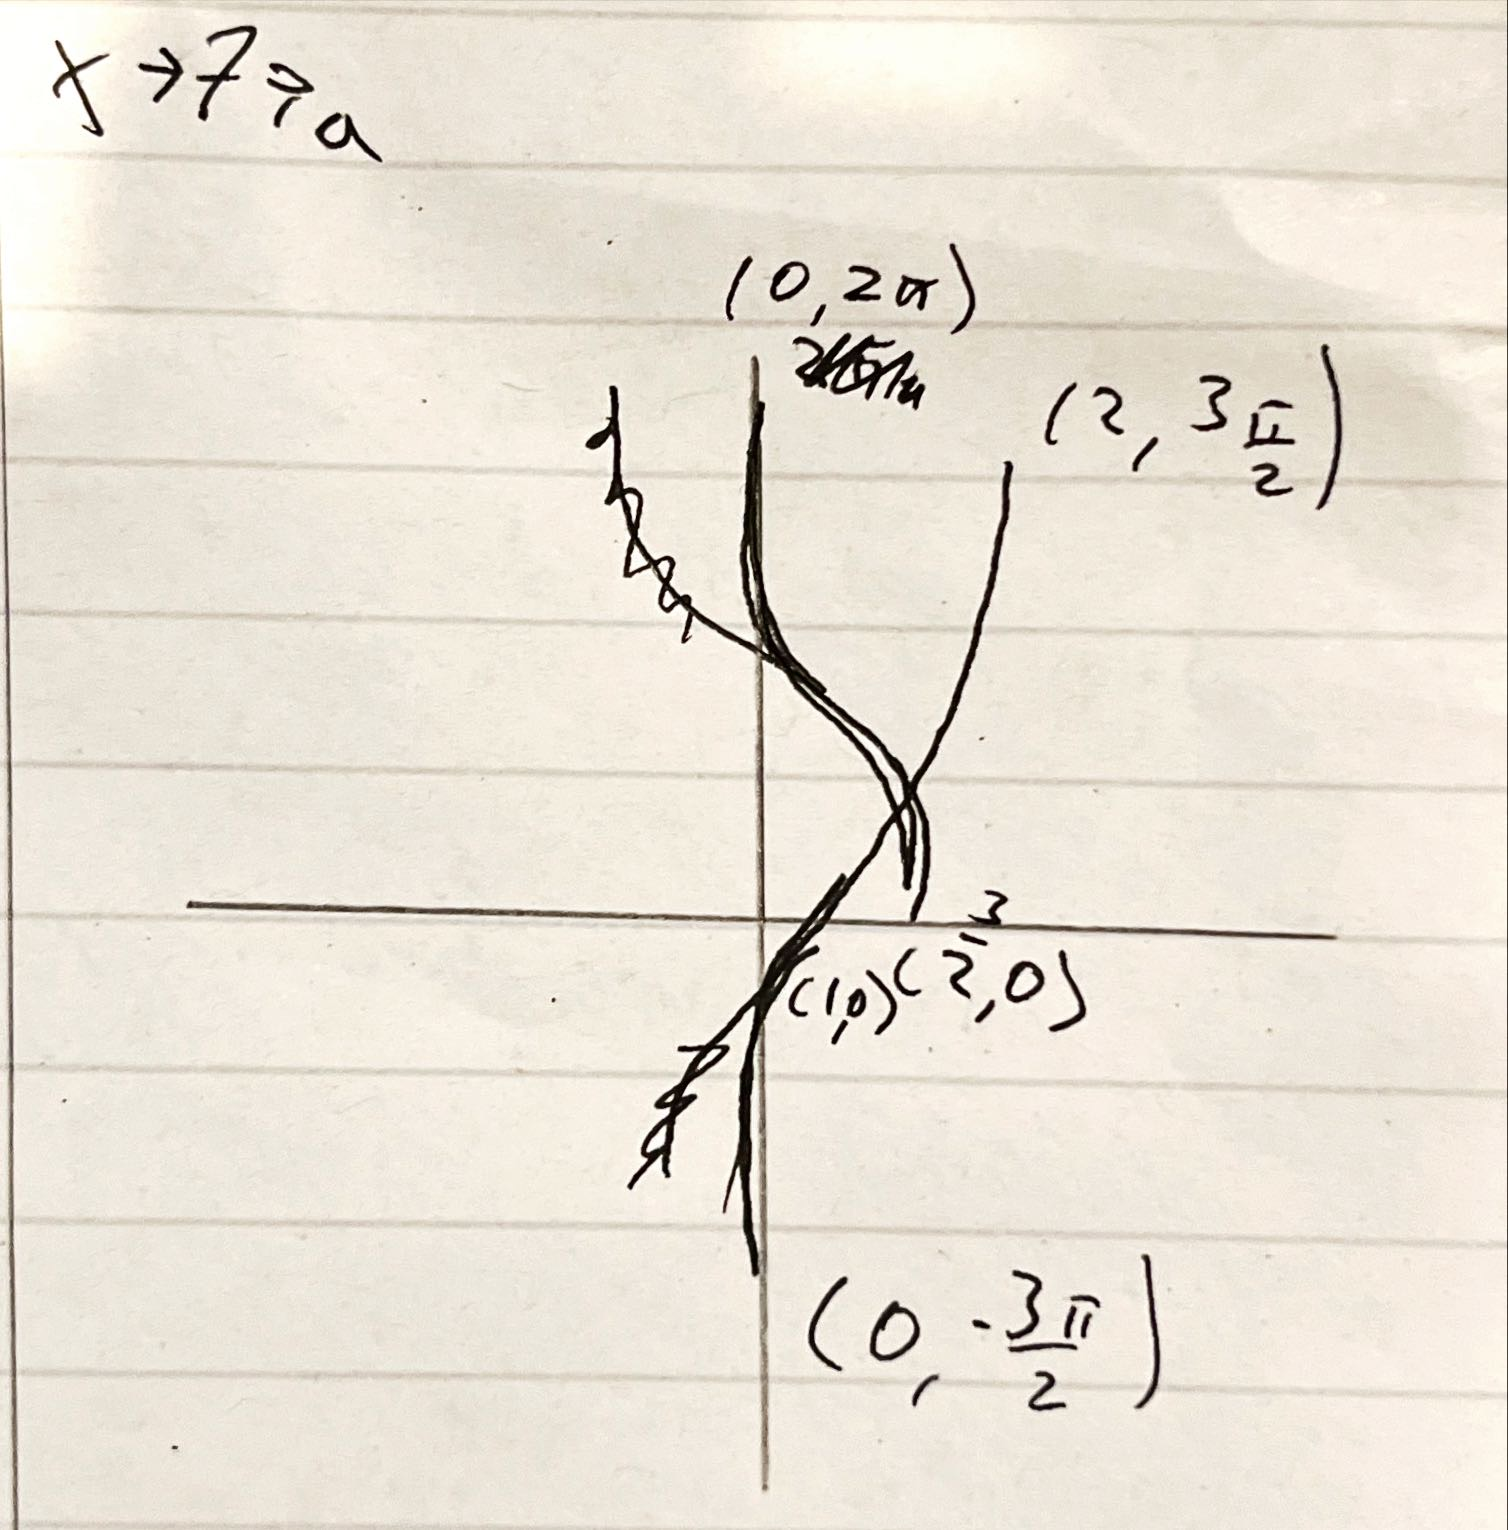
\includegraphics[width=\textwidth / 3]{y7a}
}
\qsp{b}{
	\textbf{???}
}
}

\qs{
\qsp{a}{
	\begin{align*}
		\left| \func{x} \right| &= 12 \\
		k\left( x^2 - 4x \right) &= \pm 12 \\ 
		12 / 4 &= 3 \\
		k &= 3 \\ 
		\textbf{Clarification?} &
	\end{align*}
}
\qsp{b}{
	\begin{multicols}{2}
		\noindent
		\begin{align*}
			3 \left( x^2 - 4x \right) &= 12 \\
			x^2 - 4x - 4 &= 0 \\
			x &= 2 \pm 2 \sqrt{2}
		\end{align*}
		\columnbreak
		\begin{align*}
			-3 \left( x^2 - 4x \right) &= 12 \\
			x^2 - 4x + 4 &= 0 \\
			(x-2)^2 &= 0 \\
			x &= 2
		\end{align*}
	\end{multicols}
	\[ x = 2-2\sqrt{2} \quad 2 \quad 2+2\sqrt{2} \]
}
}

	
\end{document}